\chapter{Designing a Language for Expressing Commonalities 
    \pgsize{15 p.}
}
\label{chap:language}

\todo{Grafik für die Zusammenhänge: Ansatz/Sprache bekommt konkrete Metamodelle + Commonalities-Spezifikation als Eingabe, erzeugt daraus Konzeptmetamodelle und Transformationen, die dann zur Laufzeit ausgeführt werden und Konzeptmodelle und konkrete Modelle erzeugen.}

Say that we focus on concepts and design options for language, not on concrete realization. Refer to Joshua, Lukas for that.
Depict a grammar for the overall structure to show how manifestations are embedded, commonalities are defined and related. Refer to operator concept as imaginary language element for assigning values.

Design Options: Commonalities specification

\begin{figure}
    \centering
    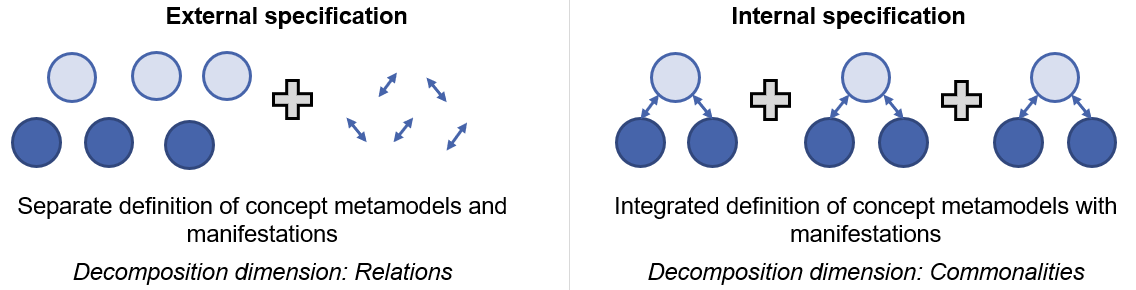
\includegraphics[width=\textwidth]{figures/quality/language/design_options.png}
    \caption[Design options for \commonalities specification]{Exemplification of alternatives to specify \commonalities by means of an integrate definition of \conceptmetamodels and manifestation relations or their separate specification.}
    \label{fig:language:design_options}
\end{figure}

Benefits of internal: easy to add commonalities + improved locality / conciseness
Drawbacks of internal: more difficult to add metamodels


\subsection*{Improving Comprehensibility}

\begin{figure}
    \centering
    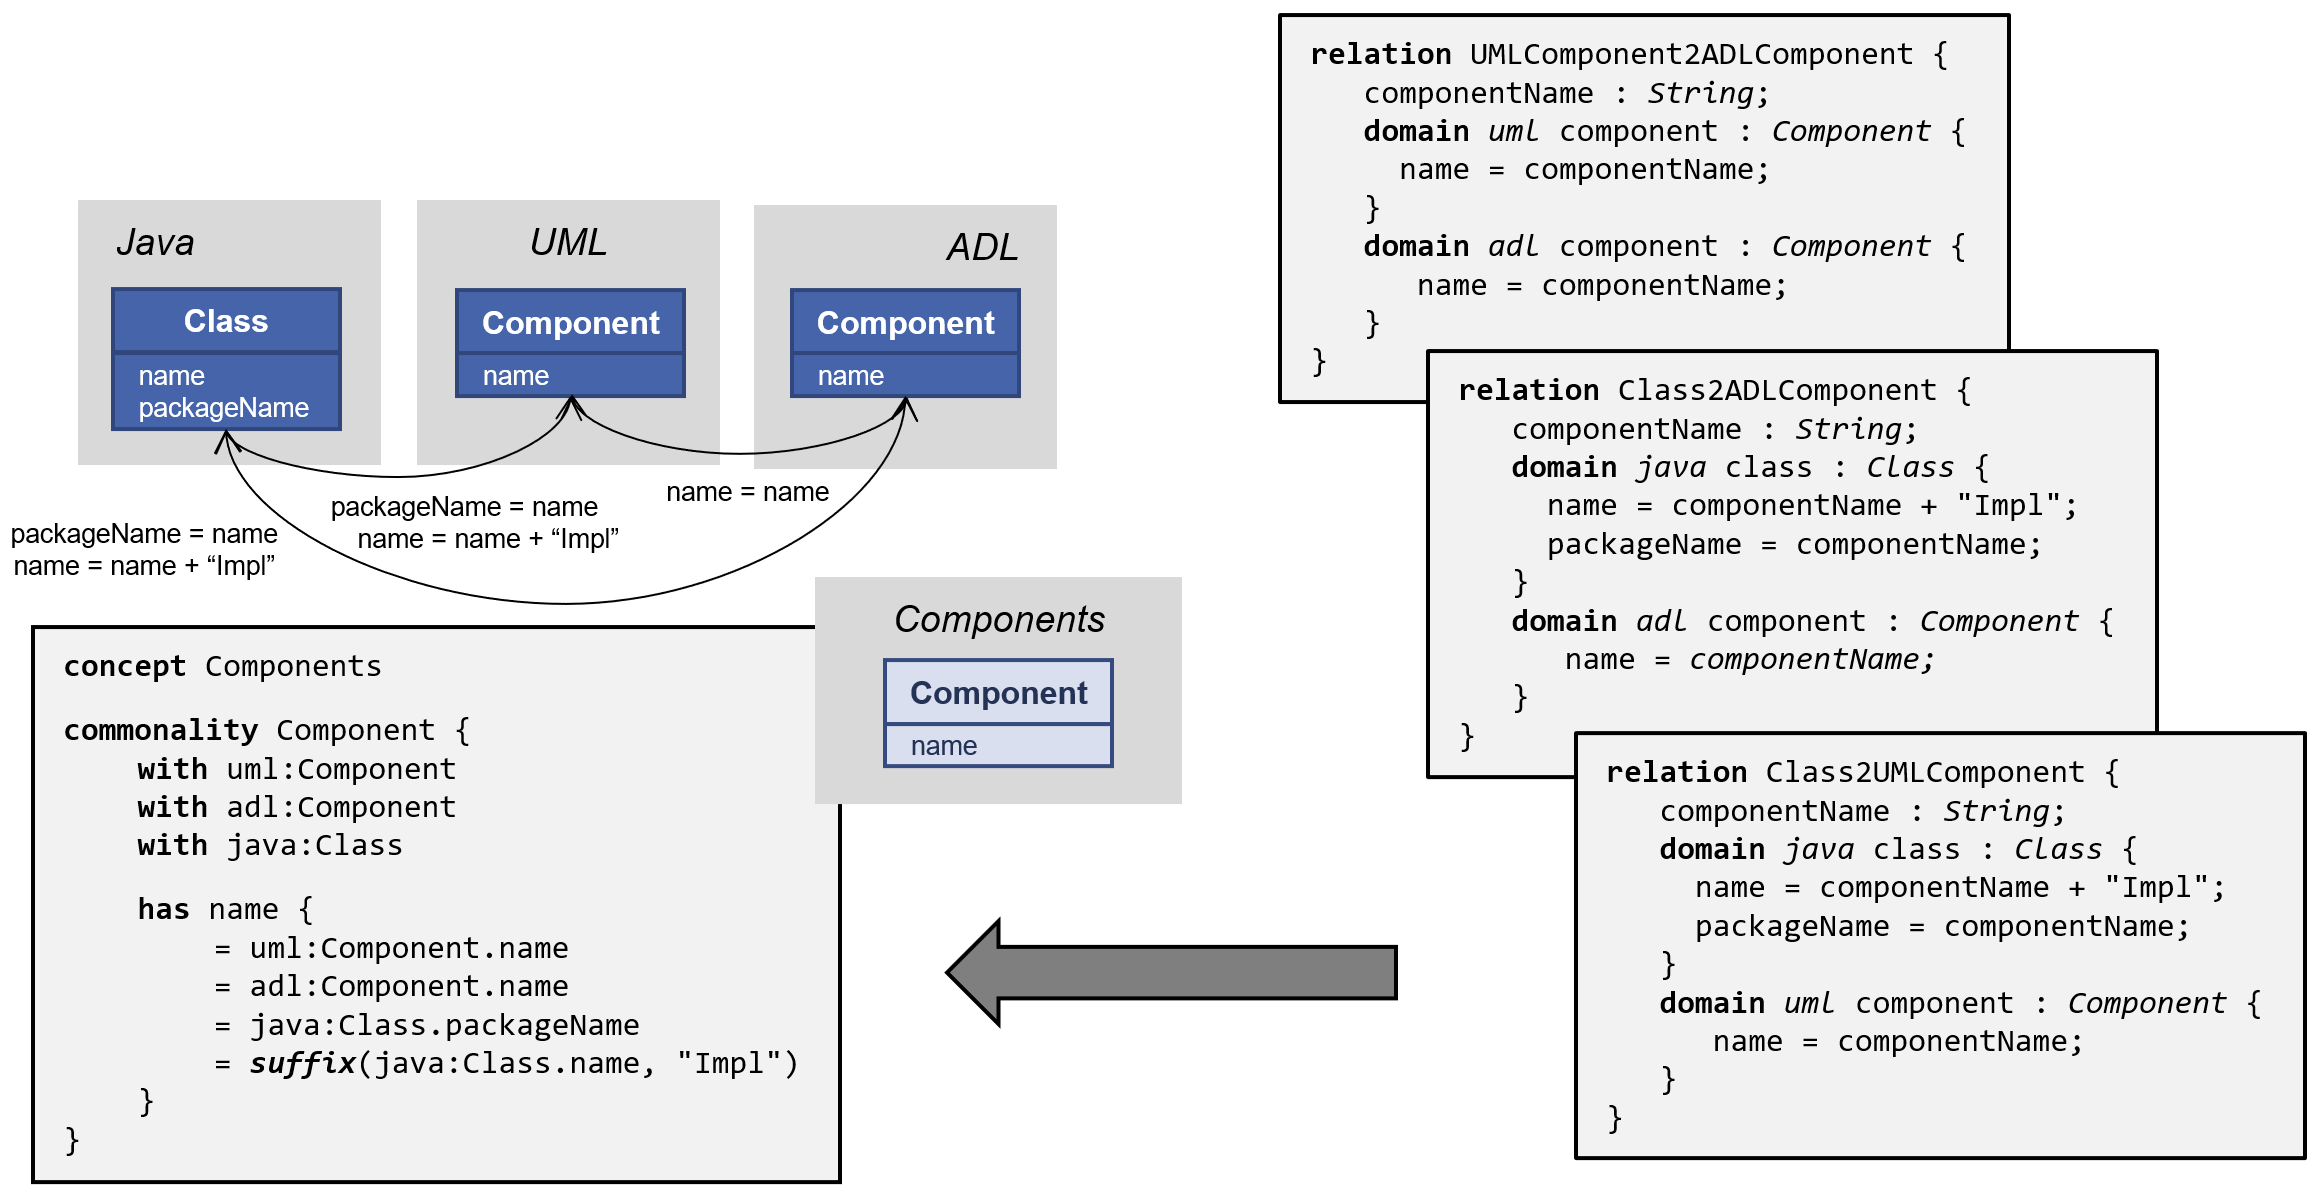
\includegraphics[width=\textwidth]{figures/quality/language/benefit_comprehensibility.png}
    \caption[Benefit of \commonalities regarding comprehensibility]{Example for consistency relations between classes and components expressed with \qvtr and the \commonalities approach.}
    \label{fig:language:benefit_comprehensibility}
\end{figure}


Further benefit: Specification effort, adding concrete metamodel, adapting commonality, easier with internal specification

\begin{copiedFrom}{VoSE}

In this paper, we present the \emph{\commonalities approach}. %, which is based on the Bachelor's thesis of \textcite{gleitze2017a}.
% Vorschlag:
It defines \commonalities between metamodels explicitly and thereby allows to state clearly which common concepts they share.
%, instead of encoding this information implicitly in a transformation.
%The approach aims to explicitly define commonalities of metamodels for describing their consistency relations rather than implicitly encoding them in a transformation.
From such a specification, transformations are derived that keep instances of those metamodels consistent.
We discuss options how to derive such transformations, strategies to hierarchically compose \commonalities, as well as benefits and limitations of the approach.
Additionally, we discuss design options for a language that supports the specification of \commonalities and present the \emph{\commonalities language}, which we have developed as a proof-of-concept.
It is based on the Bachelor's thesis of \textcite{gleitze2017a}.

Having introduced the concepts of the \commonalities approach, we now present the \commonalities language, as proposed by \textcite{gleitze2017a}.
The language is a prototypical realization of the approach.
We discuss design options for such a language and outline its syntax and its usage.
This forms our contribution~\autoref{contrib:quality:language}.
For a detailed discussion of the language capabilities, we refer to \cite{gleitze2017a}.
In this paper, we focus on the presentation of fundamental concepts  and therefore only outline the language to give an impression of what our proof-of-concept evaluation is based on.


\section{Design Options}

The development of a language for realizing the \commonalities approach provides at least two areas of design options.
First, there are different possibilities to operationalize the approach, which covers decisions that are not visible to the user of the language.
Second, different options regarding how to specify \conceptmetamodels and their relations to their manifestations exist, which are decisions that are visible to the user of the language.

We already discussed in \autoref{chap:improvement:commonalities:operationalization} that there are two different options for operationalizing a specification of \commonalities: one that uses instances of the concept metamodels and defined transformations at runtime, and one that generates direct transformations between the \concretemetamodels from the specification.
Since the way a specification is operationalized does not affect the user of the approach, it is up to the language and its designer to choose one of the options.
We chose to build a language following the former approach, because it does not limit the possible relations that can be expressed.
%We chose to build a language following the former approach, because it produces less initial effort to achieve a proof-of-concept that can be used to validate whether the approach is promising at all.

Regarding the specification of \conceptmetamodels and the transformations, there are two options:
\begin{description}[leftmargin=\parindent]
    \item[External concept definition:] \Conceptmetamodels are defined as ordinary metamodels and the relations to their manifestation are defined in an individual transformation specification %, or even specifications in ordinary transformation languages, 
    for each manifestation. %$\Rightarrow$ Benefit: Each Mapping independently specifiable
    \item[Internal concept definition:] A specialized language allows to define the \conceptmetamodel and the \commonalities it consists of together with relations of all \commonalities to their manifestations. %$\Rightarrow$ Benefit: No elements accidentally missed \todoAll{Really or is there another benefit?}
\end{description}

A benefit of the first option is that the relation to each manifestation can be specified independently, which reduces dependencies between the different manifestations of one \conceptmetamodel.
Additionally, it could be realized without developing a new language. The \conceptmetamodels can be described just like any other ordinary metamodel and one can use any existing transformation language, such as QVT, for the transformation definitions.
The second option, in contrast, requires a dedicated language that enables an integrated specification of the \conceptmetamodel and its relations to manifestations.
We chose to build a language following the second option because we expect its benefits to outweigh the mentioned disadvantages.
First, it improves locality: all information about one \commonality is represented in one place.
%instead of separating the \commonality definition from the transformation specifications.
Because of that, we expect that it is easier for developers to understand the combined transformation logic concerning one \commonality.
Additionally, the \conceptmetamodel can be easily extended with this solution whenever adding a manifestation requires defining a new \commonality.
Finally, we expect that, compared to other options, grouping transformations by their \commonality reduces the possibility for developers to forget defining one or more relevant manifestations for a \commonality.
%Finally, it is easier to ensure that for all \commonalities a relation to the manifestation is defined than in the first option, where \commonality specification and relation specification are separated.
%Nevertheless, an obvious drawback of the second option in contrast to the first is that the mappings to the concrete metamodels cannot be specified independently but are tied to the Commonality definition.
%Additionally, we expect that it makes it easier to understand the semantics of a \commonality and how it relates to its manifestations.}
%and ensure that no elements are specified in the \conceptmetamodel that do have no manifestation in all relevant \concretemetamodels.


\section{Language Description}

As introduced before, our realization of the \commonalities language
%for the previously explained \commonalities approach
provides an internal concept definition and uses the \conceptmetamodels as additional metamodels in the operationalization.
An example for the syntax of the \commonalities language is depicted in \autoref{lst:quality:commonalities_language_example}.

% \begin{figure}
%     \centering
%     \todo{Potentially extend running example so that references are covered. At least, we do not have the package in the example}
%     \includegraphics[width=\columnwidth]{figures/commonalities_language_example.PNG}
%     \caption{An example for defining the common concept of components}
%     \label{fig:commonalities_language_example}
% \end{figure}

\lstinputlisting[language=commonalities, float, belowskip=-0.8 \baselineskip,
    caption={[Exemplary commonality for components]An exemplary specification of the \texttt{Component} \commonality between \gls{PCM}, UML and the object-oriented design concept in the \commonalities language},
    captionpos=b,
    label=lst:quality:commonalities_language_example,
]{listings/quality/commonalities_language_example.lst}

The language allows to define \conceptmetamodels by declaring \commonalities, each representing one commonality between different manifestations, such as the \texttt{Component} \commonality in our example.
Relations between the \conceptmetamodels and their manifestations are supposed to be specified \emph{declaratively}.
%, which is realized as a \metaclass in the \conceptmetamodel.
For every \commonality, the \metaclasses in the manifestations that realize them are specified.
In the example, the \texttt{Component} in \gls{PCM} and the \texttt{Class} in the object-oriented design \conceptmetamodel are %defined as representations of
related to the \texttt{Component} \commonality.
In our language, a \commonality is realized by a \metaclass in the metamodel that is generated for a concept, so the \texttt{Component} \commonality is realized by a \texttt{Component} \metaclass.

Within a \commonality, attributes and references can be defined, similar to an ordinary \metaclass.
The relations of an attribute to the manifestation are declared directly at the attribute.
In the example, a \texttt{name} attribute is specified, which maps to the name of the component in \gls{PCM} and the name appended with an \enquote{Impl} suffix in Java.
The language %defined by \textcite{gleitze2017a} 
provides several operators for attribute relations, apart from equality relations.
The example depicts a prefix operator that allows to compose a String attribute.
Such operators can be defined independently and added to the language dynamically.
References can be defined comparably to attributes but can be enriched with a definition of containment relations.

% Introduce the idea of \enquote{Concepts} and \enquote{Commonalities}, explain how attributes and references are mapped.
% \todo{We have to align the definition of Concept, Commonality etc. in the paper with the implementation}

The actually conceptualized and implemented language by \textcite{gleitze2017a} is far more sophisticated than the simple overview we provide here. 
It supports different kinds of bidirectional operators for attribute mappings, containment specifications (so-called \emph{participations}), attribute checks as preconditions for \commonality instantiation, and more.

\end{copiedFrom} % VoSE
